 
 \newpage
%\clearpage
\pagenumbering{arabic}
%\setcounter{page}{13}
 
 
%\addcontentsline{toc}{chapter}{ \hfill 12}
 
 \addtocontents{toc}{\protect\contentsline{chapter}{CAPÍTULO I. Generalidades del diseño térmico y cámaras de refrigeración de insulina \hfill 12}{}{}}
 


\begin{titlepage}
 
	
	
	\centering
	\begin{tikzpicture}%opacity=0.5
		\node[inner sep=0pt, ] (image) at (0,0) {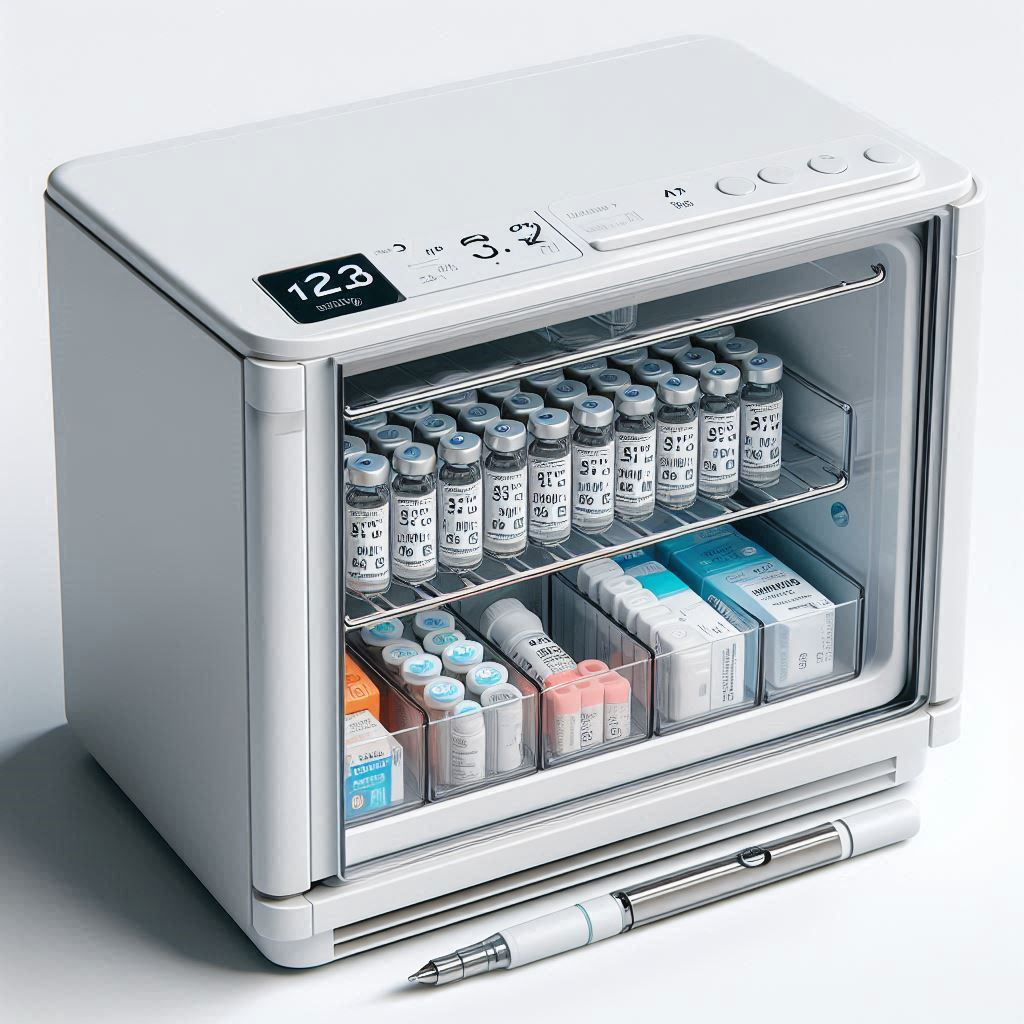
\includegraphics[width=\textwidth]{figures/bg-cap1}};
		\fill [white,path fading=south] (-5,-4) rectangle (5,4);
		\node[black,font=\Huge\bfseries] at (0,3) {Capítulo I};
		\node[black,font=\Huge\bfseries] at (0,2) {Antecedentes históricos};
				
		\node[black,font=\LARGE\bfseries] at (0,0.8) {Generalidades del diseño térmico y};
		\node[black,font=\LARGE\bfseries] at (0,-0.4) {cámaras de refrigeración de insulina};
	\end{tikzpicture}
\end{titlepage}

 

\newpage 

\section*{Introducción}


\addcontentsline{toc}{section}{{Introducción}}\rsp
\setcounter{chapter}{1}
 \setcounter{page}{13}


La refrigeración no es más que el proceso en el que se elimina el calor contenido en un espacio cerrado para excluirlo a una temperatura más alta, es decir técnicamente se está trasladando calor de una temperatura relativamente baja a una más alta \cite{Hundy1984}.

En países industrializados la refrigeración tradicionalmente se ha empleado para preservar alimentos a temperaturas bajas, lo que impide la proliferación de bacterias, levaduras y moho que pueden causar su deterioro. Esto posibilita la congelación de muchos productos perecederos, lo que permite su conservación durante largos periodos, incluso meses o años, sin una considerable pérdida de valor nutricional, sabor o alteración en su apariencia \cite{britannica2023}.

De acuerdo con \citeauthor{khurana2019}, \citeyear{khurana2019}, la insulina es una hormona endógena que se produce de manera natural por el páncreas. La función principal radica en facilitar la absorción y utilización de la glucosa por parte de las células del cuerpo. Esta glucosa sirve como fuente de energía para las diversas funciones celulares en el cuerpo humano. Las personas con \textit{diabetes mellitus} (DM) experimentan una disminución en la capacidad para absorber y utilizar la glucosa en la sangre, lo que resulta en un aumento de los niveles de glucosa en la misma. En el caso de la diabetes tipo 1, el páncreas no produce suficiente insulina, lo que requiere tratamiento con terapia de insulina. Por otro lado, en la diabetes tipo 2, los pacientes producen insulina, pero las células de su cuerpo no responden adecuadamente a ella, lo que se conoce como resistencia a la insulina. Aunque la insulina se utiliza comúnmente en el tratamiento de la diabetes tipo 1, también puede ser recetada para pacientes con diabetes tipo 2 para superar la resistencia a la insulina. 

\newpage

\section{Las cámaras de refrigeración a través de la historia}

La práctica de la refrigeración, a menudo asociada con tecnología moderna, tiene sus raíces en tiempos antiguos, donde la preservación de alimentos era crucial. Desde la antigüedad, los seres humanos han recurrido a métodos naturales, como almacenar alimentos en cuevas frescas o utilizando hielo de montañas para mantenerlos frescos, vea la figura \ref{fig:pozo-nieve} de un ejemplo situado la Mancomunidad Turística de Sierra Espuña. Este enfoque permitía tener reservas alimenticias disponibles en tiempos de necesidad. Además, desde el siglo XVI, se ha empleado la técnica de mezclar hielo con sal para lograr temperaturas por debajo de su punto de fusión, destacando la continua búsqueda de soluciones para la conservación de alimentos en condiciones adversas. (UPV, 2020)

\begin{figure}[H]
	\centering
	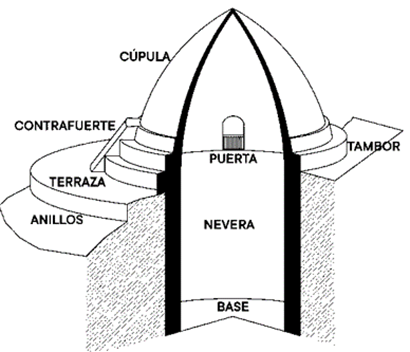
\includegraphics[width=0.6\linewidth]{figures/pozo-nieve}
	\caption{Esquema de las partes principales de un pozo de nieve}
		Fuente: \cite{ecoproyecta2024}
	\label{fig:pozo-nieve}
\end{figure}

\subsection{Época antigua}

Durante siglos, se ha tenido conocimiento de que la evaporación del agua genera una sensación de frescor. En épocas antiguas, aunque no se buscaba comprender el fenómeno, se observaba que cualquier parte del cuerpo mojada se enfriaba al secarse al aire. Ya en el siglo II, en Egipto se empleaba la evaporación para enfriar jarras de agua, mientras que en la antigua India se utilizaba para la producción de hielo (Neuberger, 1930).


\subsection{Grecia y el imperio romano}
En la antigua Grecia e Imperio Romano, se desarrollaron ingeniosos métodos de refrigeración que se basaban en el aprovechamiento de la nieve y el hielo. Griegos y romanos contaban con una comprensión rudimentaria de cómo preservar alimentos en climas cálidos, utilizando nieve de montañas y áreas frías. Uno de estos métodos implicaba cavar hoyos en la tierra y forrarlos con aislantes naturales como paja y ramas, donde se almacenaba cuidadosamente nieve o hielo recolectados en invierno, manteniendo una temperatura baja y conservando alimentos perecederos como carnes y pescados durante las estaciones más calurosas del año.

Esta práctica se difundió por el Mediterráneo y otras regiones donde las altas temperaturas planteaban desafíos para la conservación de alimentos, convirtiéndose en una técnica esencial para comunidades rurales y empleada ampliamente hasta el siglo XX  \cite{jr2013}.

\subsection{Época media}
Durante la Edad Media, surgieron técnicas innovadoras de refrigeración en la India del siglo IV y en la Península Ibérica bajo el gobierno musulmán, donde se utilizaban procesos químicos como la disolución de nitrato sódico y nitrato de potasio en agua para bajar la temperatura, representando un avance significativo en la tecnología de refrigeración. En el siglo XVI, Blas Villafranca, un médico español en Roma, experimentó con la refrigeración de líquidos como agua y vino mediante mezclas refrigerantes. Sin embargo, el descubrimiento más impactante ocurrió en 1607, cuando se descubrió que una combinación de agua y sal tenía la capacidad de congelar el agua, revolucionando la producción de hielo artificial y transformando la conservación de alimentos y la refrigeración en una época donde las altas temperaturas presentaban desafíos continuos.

Estos avances en la refrigeración artificial durante la Edad Media marcaron un hito en la evolución de la tecnología de conservación de alimentos y bebidas en condiciones climáticas adversas \cite{bernad2023}.

\subsection{Época contemporánea}

Según estudios reportados de Goosman en el año 1924, los primeros intentos de crear refrigeración mecánica se basaron en los efectos refrigerantes de la evaporación del agua. En 1755, William Cullen, un médico escocés, logró obtener temperaturas lo suficientemente bajas como para producir hielo. Esto lo logró al reducir la presión del agua en un recipiente sellado mediante una bomba de aire. Bajo una presión muy pequeña, el agua se evaporaba o hervía a una temperatura baja, extrayendo calor del resto del agua y provocando la formación de hielo. Desde Cullen, numerosos ingenieros y científicos han creado una variedad de inventos para comprender los principios básicos de la refrigeración mecánica \cite{dincer2010}.

Según indican \cite{critchell1912}, en el año 1834, Jacob Perkins, un ciudadano estadounidense viviendo en Inglaterra, diseñó y obtuvo la patente de una máquina que empleaba compresión de vapor, que incluía un compresor, un condensador, un evaporador y un grifo situado entre el condensador y el evaporador. A continuación en la figura \ref{fig:aparato-jacob} se muestra el aparato diseñado por Perkins en donde se aprecia que el refrigerante (éter u otro fluido volátil) hierve en el evaporador B tomando calor del agua circundante en el recipiente A. La bomba C extrae el vapor y lo comprime a una presión más alta a la que puede condensarse a líquidos en los tubos D, cediendo calor al agua en el recipiente E. El líquido condensado fluye a través de la válvula cargada de peso H, que mantiene la diferencia de presión entre el condensador y el evaporador. La pequeña bomba situada encima de H se utiliza para cargar el aparato con refrigerante.

\begin{figure}[H]
	\centering
	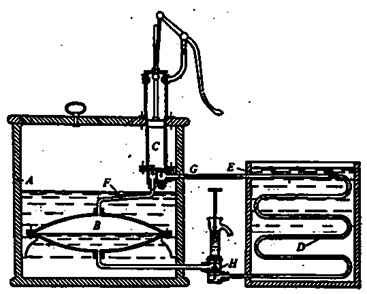
\includegraphics[width=0.6\linewidth]{figures/aparato-jacob}
	\caption{Aparato de Jacob Perkins en la especificación de su patente de 1834}
	Fuente: \cite{vidyaputra}.
	\label{fig:aparato-jacob}
\end{figure}

 
Durante las tres décadas posteriores a 1850, la creciente demanda impulsó una ola de innovación y progreso. Científicos destacados como Faraday y Thilorier introdujeron nuevas sustancias, como el amoníaco y el dióxido de carbono, que demostraron ser más eficaces que el agua y el éter, incluso pudiendo ser licuadas. Este avance fue respaldado por un sólido fundamento teórico proporcionado por Rumford y Davy, quienes habían esclarecido la naturaleza del calor, y por científicos como Kelvin, Joule y Rankine, quienes ampliaron el trabajo iniciado por Sadi Carnot en la formulación de la ciencia de la termodinámica, sentando así las bases para la refrigeración mecánica.

\section{El origen de la refrigeración en China y su desarrollo en occidente.}
La historia de la refrigeración se remonta a la antigua China, donde se descubrió por primera vez el potencial de la salmuera para enfriar alimentos. En el siglo XIV, Marco Polo trajo consigo desde China a Occidente el conocimiento sobre la fabricación de sorbetes de leche, que se cree se basaba en el principio de la evaporación de la salmuera. Los chinos, que utilizaban la salmuera para preservar alimentos, probablemente observaron sus propiedades refrigerantes \cite{curiosfera2023}. 

En torno al año 1660, el italiano Zimara propuso utilizar una combinación de nieve y salitre como agente refrigerante. Posteriormente, de forma empírica, se observó que la rápida evaporación de la salmuera caliente provocaba la absorción de calor. Este proceso, influenciado por las ideas de Zimara y por el uso de alcarrazas turcas (recipientes de barro poroso que mantenían el agua fresca mediante la evaporación), sentó las bases en el siglo XVII para los primeros intentos de refrigeración controlada en Occidente. Así, la historia de la refrigeración comenzó en China y gradualmente se difundió por todo el mundo, influyendo en el desarrollo de técnicas y tecnologías de conservación de alimentos inicialmente, hoy en día estas aplicaciones son extensas (Atecyr, 2020)

\section{Historia de la insulina y su preservación}
El 12 de diciembre de 1921 Banting y Best descubrieron la insulina, que nació como una posible esperanza de cura. Al año siguiente, Leonard Thompson, un niño de 14 años con diabetes severa, fue el primer paciente al que se le aplicó una inyección de extracto pancreático vacuno (Vecchio et.al, 2018).

De acuerdo a Buse JB, Davies MJ, Frier BM, et al 100 years on: the impact of the discovery of insulin  (2021), hasta comienzos del siglo pasado la diabetes representaba un trastorno devastador, especialmente cuando se diagnosticaba en la infancia, ya que solía resultar mortal. Por lo tanto, el exitoso descubrimiento y extracción de insulina a partir del páncreas en 1921 marcó un avance maravilloso que transformó radicalmente la vida de quienes padecían esta enfermedad. En la figura \ref{fig:nino1diabetes} se aprecia a un niño el cual era un paciente de diabetes tipo 1, antes de ser medicado de insulina y obtener los beneficios de la hormona dejando de lado la rigurosa ingesta de calorías en los centros médicos de aquellos tiempos.

\begin{figure}[H]
	\centering
	\includegraphics[width=0.6\linewidth]{figures/niño1diabetes}
	\caption{Fotos de antes y después de un niño con diabetes tipo 1.}
	Fuente: \cite{novo}
	\label{fig:nino1diabetes}
\end{figure}

\subsection{Medidas preventivas de la insulina}
La insulina, al ser una proteína, puede sufrir cambios y perder su eficacia. Es especialmente vulnerable a la precipitación causada por alteraciones en el pH y la temperatura. Estos cambios físico químicos pueden provocar su degradación tanto física (cambios en su estado físico sin alterar su estructura covalente) como química (alteraciones en su estructura covalente). Por ello, es crucial almacenar los viales de insulina sin abrir en un ambiente controlado entre 2 y 8°C, protegidos de la luz \cite{khurana2019}.

Los productos de insulina, ya sea en frascos o cartuchos proporcionados por los fabricantes, pueden mantenerse sin refrigeración a temperaturas entre 15 °C y 30 °C durante un máximo de 28 días y seguir siendo efectivos, tanto si están abiertos como si no. Sin embargo, cualquier insulina que haya sido modificada para diluirse o que se haya extraído del envase original del fabricante debe desecharse en un plazo de dos semanas. Cuanto más prolongada sea la exposición a estas temperaturas, menor erá su eficacia, lo que puede conducir a una pérdida de control de la glucosa en la sangre con el tiempo. 

\subsection{Preservación de la insulina}

Las primeras formas de almacenamiento y preservación de la insulina para mantener estable su capacidad y eficacia fueron a través de jeringas. Las primeras jeringas de vidrio fabricadas por Becton Dickinson eran pesadas y frágiles, con agujas largas y gruesas que requerían esterilización mediante ebullición antes de ser reutilizadas. En 1954, se introdujo la primera jeringa desechable de vidrio, seguida por una versión de plástico en 1955. Estas jeringas, estaban equipadas con agujas integradas o desechables hacían que las inyecciones fueran menos dolorosas, pero aún presentaban problemas de dosificación. La jeringa de insulina U100, hecha de un plástico especial con unidades marcadas, mejoró la precisión y permitió una reutilización segura. Avances posteriores incluyeron agujas de calibre más corto para minimizar el dolor, aunque persistieron problemas de precisión en la dosificación \cite{buse2021}.

\subsection{Refrigeración de la insulina. }

Como indica en su artículo Smith, J. (2020), la modernización de la refrigeración de la insulina ha sido un proceso gradual que ha ido evolucionando en paralelo con los avances tecnológicos y científicos. Inicialmente, la conservación de la insulina dependía de métodos básicos como el almacenamiento en lugares frescos o en recipientes con hielo. Sin embargo, a medida que avanzaba el tiempo, se produjeron mejoras significativas en este campo. Con el desarrollo de la tecnología en la década de 1920, se introdujeron los primeros refrigeradores domésticos, lo que permitió un almacenamiento más seguro en los hogares\footnote{A principios del siglo XIX, los inventores estadounidenses Oliver Evans, Jacob Perkins y John Gorrie desarrollaron las primeras versiones del frigorífico moderno}. 

El autor también describe que estos primeros modelos eran bastante simples y proporcionaban un ambiente fresco, pero carecían de un control preciso de la temperatura. A lo largo del siglo XX, con el avance tecnológico, se diseñaron refrigeradores más sofisticados con controles de temperatura precisos, específicamente adaptados para almacenar medicamentos sensibles como la insulina. En las últimas décadas, se han desarrollado refrigeradores portátiles y dispositivos de almacenamiento compactos, lo que ha proporcionado a los pacientes con diabetes una forma conveniente y segura de transportar su insulina. Estos dispositivos suelen estar equipados con tecnología avanzada de control de temperatura y funciones de monitoreo para garantizar la integridad del medicamento.

\subsection{Avances tecnológicos en la refrigeración de la insulina}

Durante la última década, ha habido avances significativos en la tecnología utilizada para tratar la diabetes. Hoy en día disponemos de dispositivos de infusión continua de insulina subcutánea o bombas de insulina que intentan imitar la secreción fisiológica del páncreas, así como de monitorización continua de la glucosa que proporciona información de la glucosa intersticial las 24 horas del día. Los modelos más modernos combinan ambas tecnologías en un solo dispositivo e incluso son capaces de detener la infusión de insulina en caso de hipoglucemia (Apablaza et al., 2016). 

De acuerdo a una modificación de la imagen dada por MedlinePlus, 2024, en Estados Unidos a través de su sitio web oficial, la imagen \ref{fig:bomba-insul} que se muestra a continuación en la cual se observa cómo la bomba suministra insulina de manera continua. En su interior, dispone de un depósito que contiene un análogo de insulina rápida (insulina ultrarrápida), el cual se conecta a un catéter encargado de transferirla al tejido subcutáneo mediante una cánula.


\begin{figure}[H]
	\centering
	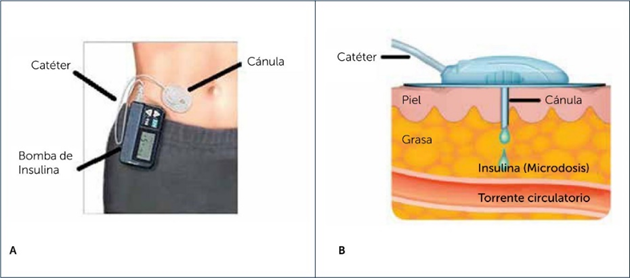
\includegraphics[width=0.7\linewidth]{figures/bomba-insul}
	\caption{Bomba de insulina y set de infusión (A), (B) posición de la Cánula en el tejido Subcutáneo}
	Fuente:\cite{apablaza-2016}
	\label{fig:bomba-insul}
\end{figure}


 
